% !TeX root = ../main.tex
\documentclass[./../main.tex]{subfiles}

\begin{document}
\subsection{Gợi ý cho người dùng các truyện nổi bật}
Thông thường, những bộ truyện mới ra mắt hoặc có lượt truy cập tiềm năng sẽ khó có thể tiếp cận đến các độc giả. Quản trị viên có thể giới thiệu những bộ truyện tới người dùng thông qua tính năng gợi ý các truyện nổi bật. Những truyện này sẽ xuất hiện ngay trên trang đầu của ứng dụng, ngay khi người dùng truy cập bằng cách tóm tắt nội dung truyện và hình ảnh bắt mắt.

\begin{figure}[!htb]
	\centering
	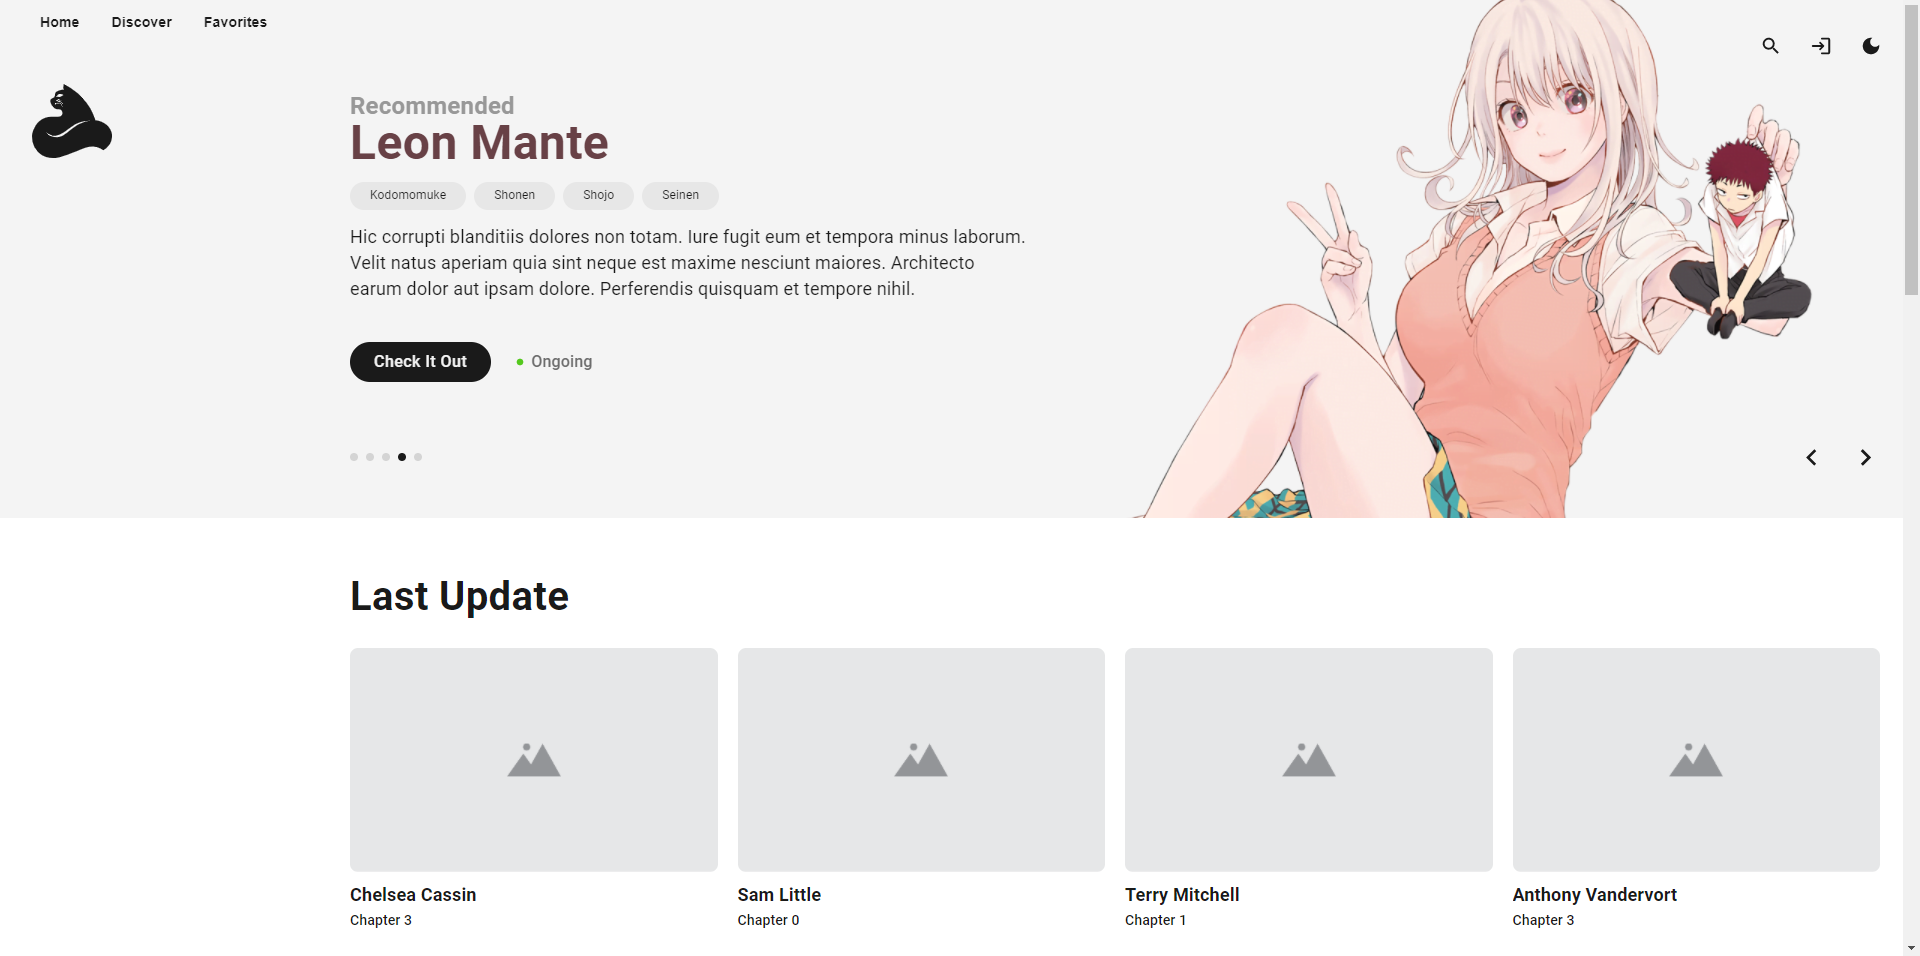
\includegraphics[width=\linewidth]{./images/recommend.png}
	\caption{Gợi ý truyện}
\end{figure}

Đây cũng là kênh marketing vô cùng hiệu quả để thu lại lượng traffic tự nhiên của người dùng về những bộ truyện nổi bật.
\subsection{Lọc danh sách truyện theo nhiều tiêu chí}
Việc tìm kiếm truyện theo danh sách là vô cùng quan trọng. Người đọc có thể dễ dàng tìm thấy những bộ truyện theo từng thể loại, tác giả, trạng thái xuất bản,... mà mình quan tâm.

\begin{figure}[!htb]
	\centering
	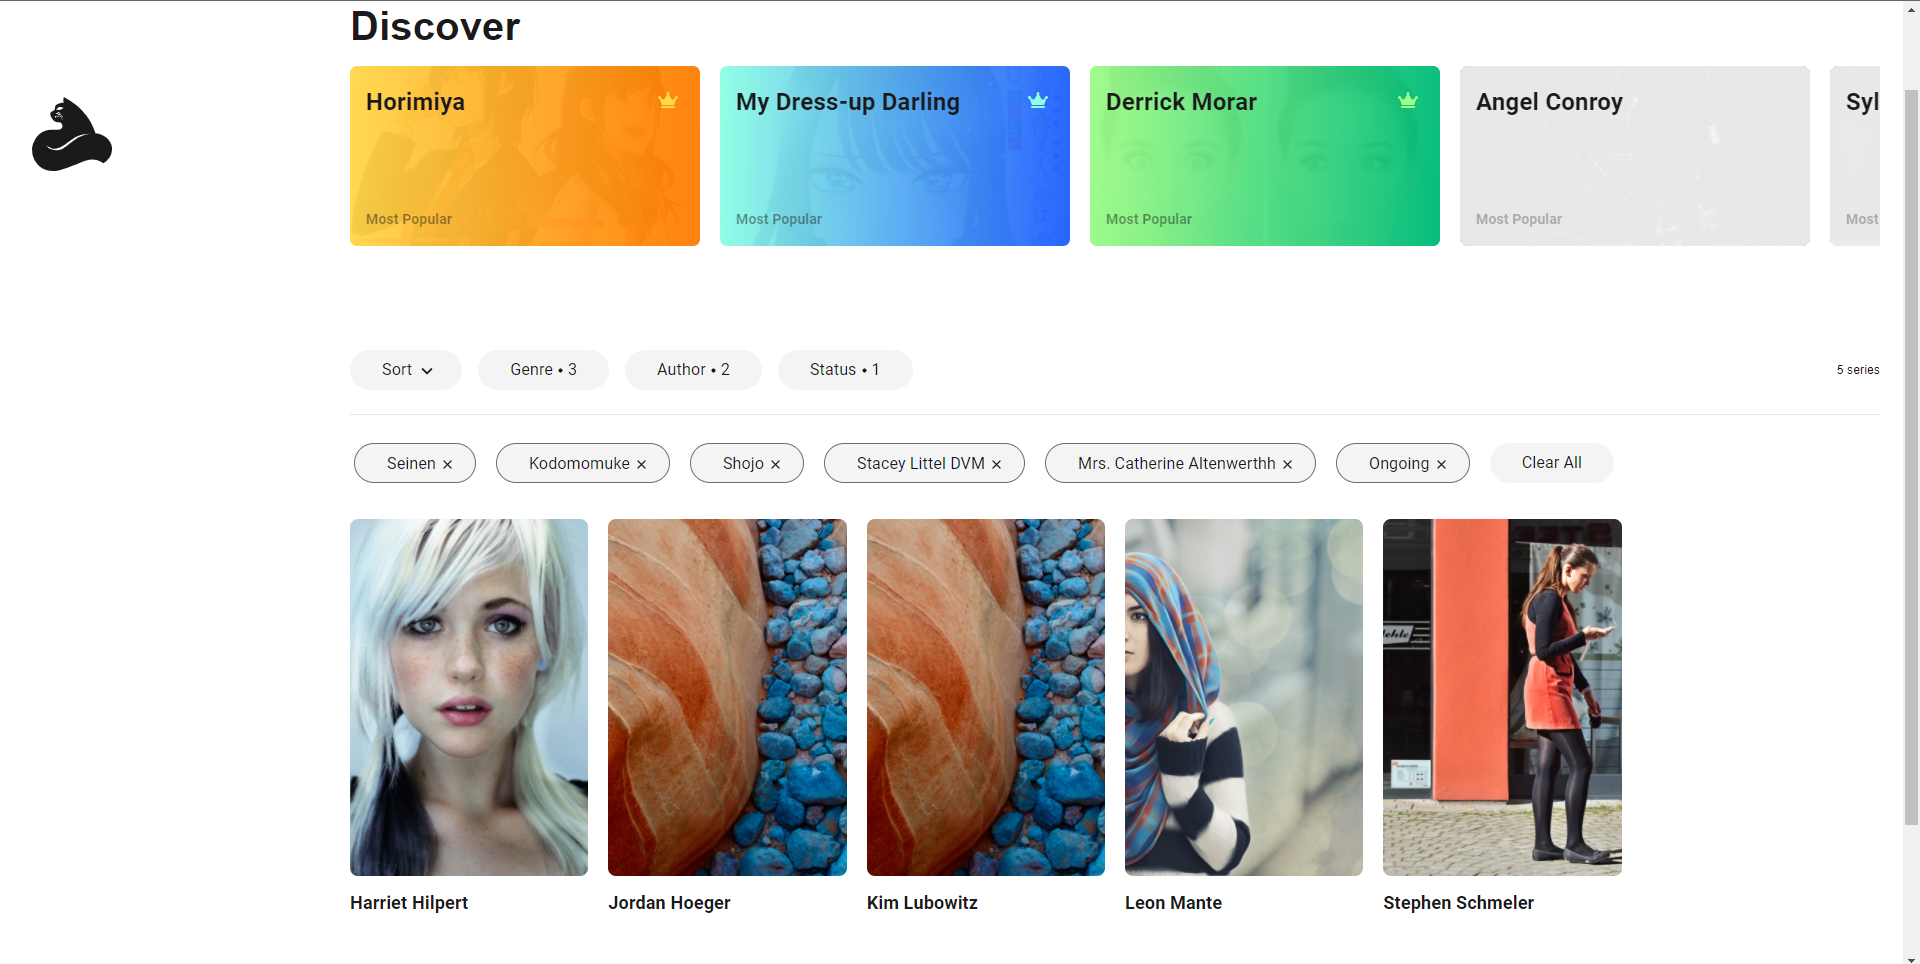
\includegraphics[width=\linewidth]{./images/filter.png}
	\caption{Lọc danh sách truyện}
\end{figure}

\subsection{Xếp hạng các truyện phổ biến nhất}
Bảng xếp hạng là nơi đánh giá những bộ truyện dựa trên mức độ phổ biến của chúng trong một khoảng thời gian nhất định. Để thấy được sự phổ biến của bộ truyện, có rất nhiều tiêu chí được đưa vào để đánh giá như số lượt truy cập, số lượt đọc truyện và số lượt bình luận.

\begin{figure}[!htb]
	\centering
	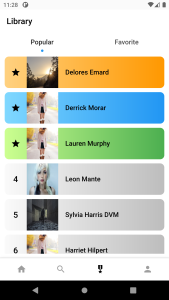
\includegraphics[width=0.5\linewidth]{./images/ranking.png}
	\caption{Xếp hạng truyện}
\end{figure}

Bảng xếp hạng góp phần quảng bá các truyện phổ biến gần đây đến trực tiếp người dùng. Những bộ truyện đứng đầu bảng xếp hạng có thể mang lại nhiều lượt truy cập và trở thành lựa chọn đáng tin cậy đối với độc giả.
\subsection{Lưu truyện vào danh sách yêu thích}
Khi số lượng truyện tăng lên theo thời gian, thật khó để tìm kiếm và đọc được truyện mà người dùng đang quan tâm. Việc lưu truyện vào trong danh sách yêu thích sẽ giúp người dùng giảm được thời gian thao tác trên ứng dụng cũng như không phải ghi nhớ chi tiết từng tên truyện mà mình yêu thích.

\begin{figure}[!htb]
	\centering
	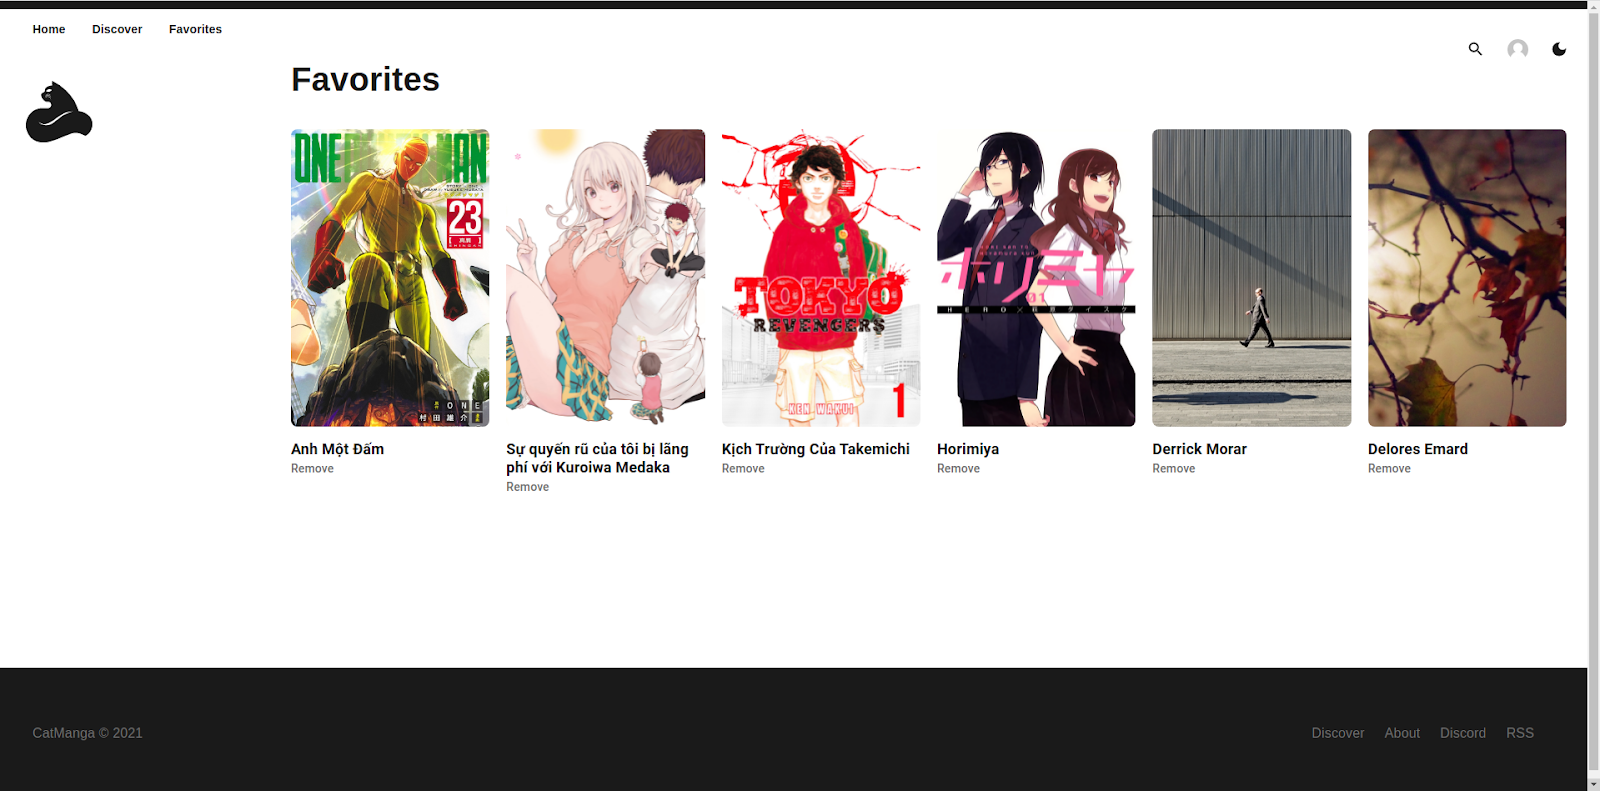
\includegraphics[width=\linewidth]{./images/favorite.png}
	\caption{Lưu truyện vào danh sách yêu thích}
\end{figure}

Sau khi đăng nhập, người dùng đã có thể chuyển sang mục “Yêu thích” chỉ với một vài thao tác đơn giản. Nếu người dùng không còn quan tâm, họ có thể xoá truyện khỏi danh sách yêu thích, truyện đó sẽ không hiển thị trong danh sách của người dùng nữa.
\subsection{Xem lịch sử đọc truyện}
Đang thưởng thức dở một bộ truyện gay cấn trên máy tính nhưng lại có việc gấp phải ra ngoài? Truyện tuần trước mới đọc xong thấy hay quá nhưng bây giờ lại quên mất tên rồi? Bạn nên để tâm trí mình cho việc khác thay vì những nỗi lo này bởi Honyomi đã cung cấp tính năng xem lại lịch sử đọc truyện.


\begin{figure}[!htb]
	\centering
	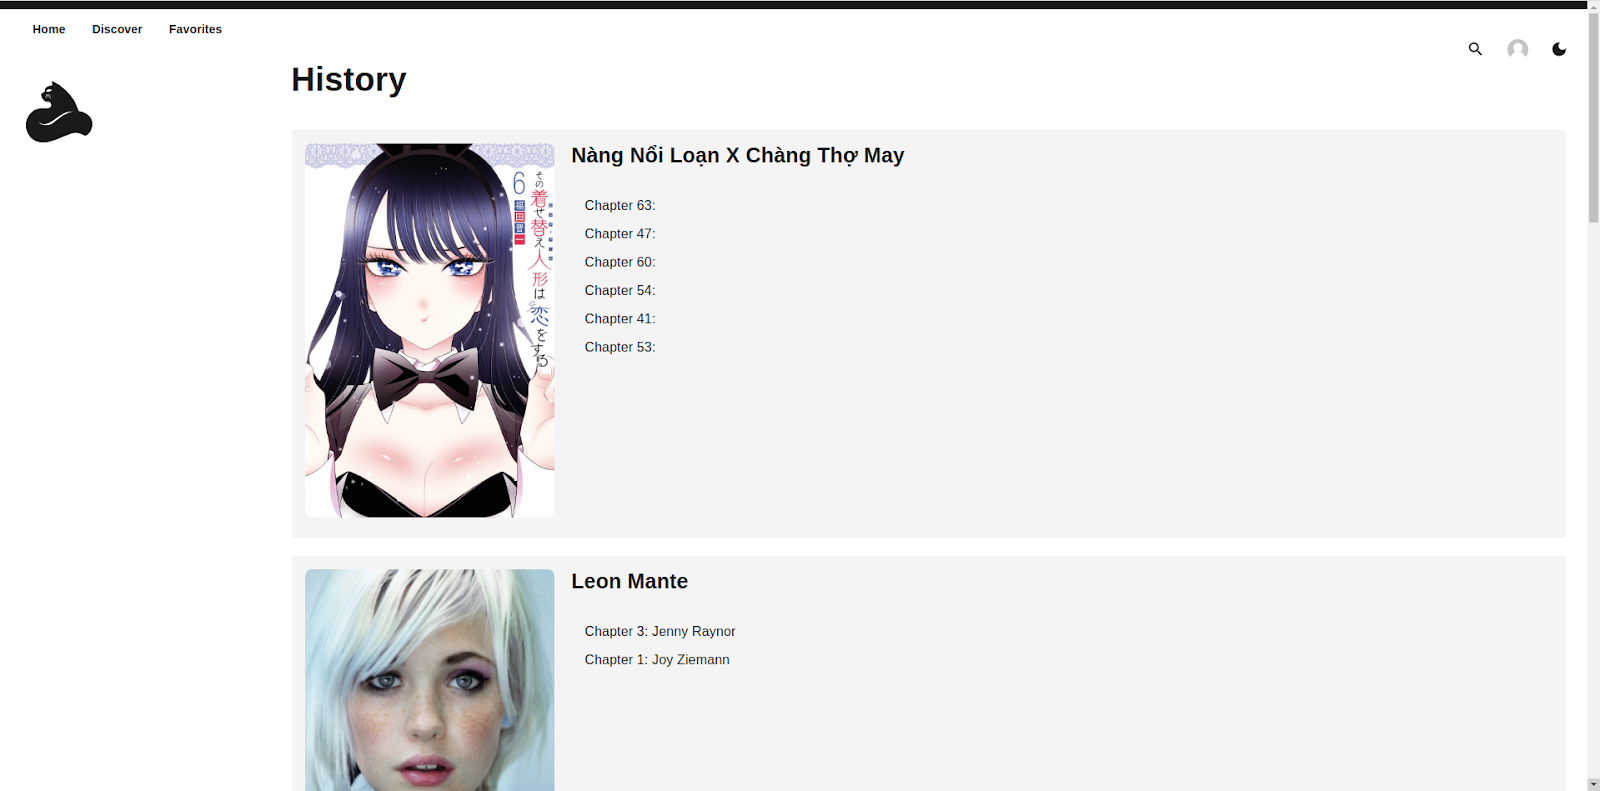
\includegraphics[width=\linewidth]{./images/history.png}
	\caption{Xem lịch sử đọc truyện}
\end{figure}

Chỉ cần đăng nhập vào hệ thống bằng bất kỳ cách nào, mọi lịch sử đọc truyện của bạn đều được lưu lại vào hệ thống và có thể tra cứu lại bất cứ lúc nào bạn muốn. Honyomi lưu trữ lịch sử của bạn lên đến 6 tháng gần đây nhất của tất cả người dùng nên bạn có thể hoàn toàn yên tâm. Còn muốn lưu trữ lâu dài hơn, bạn nên sử dụng ngay chức năng Lưu truyện vào danh sách yêu thích, truyện sẽ ở đó mãi mãi cho đến khi bạn hết yêu thích.
\subsection{Đăng nhập với tài khoản Google}

\begin{figure}[!htb]
	\centering
	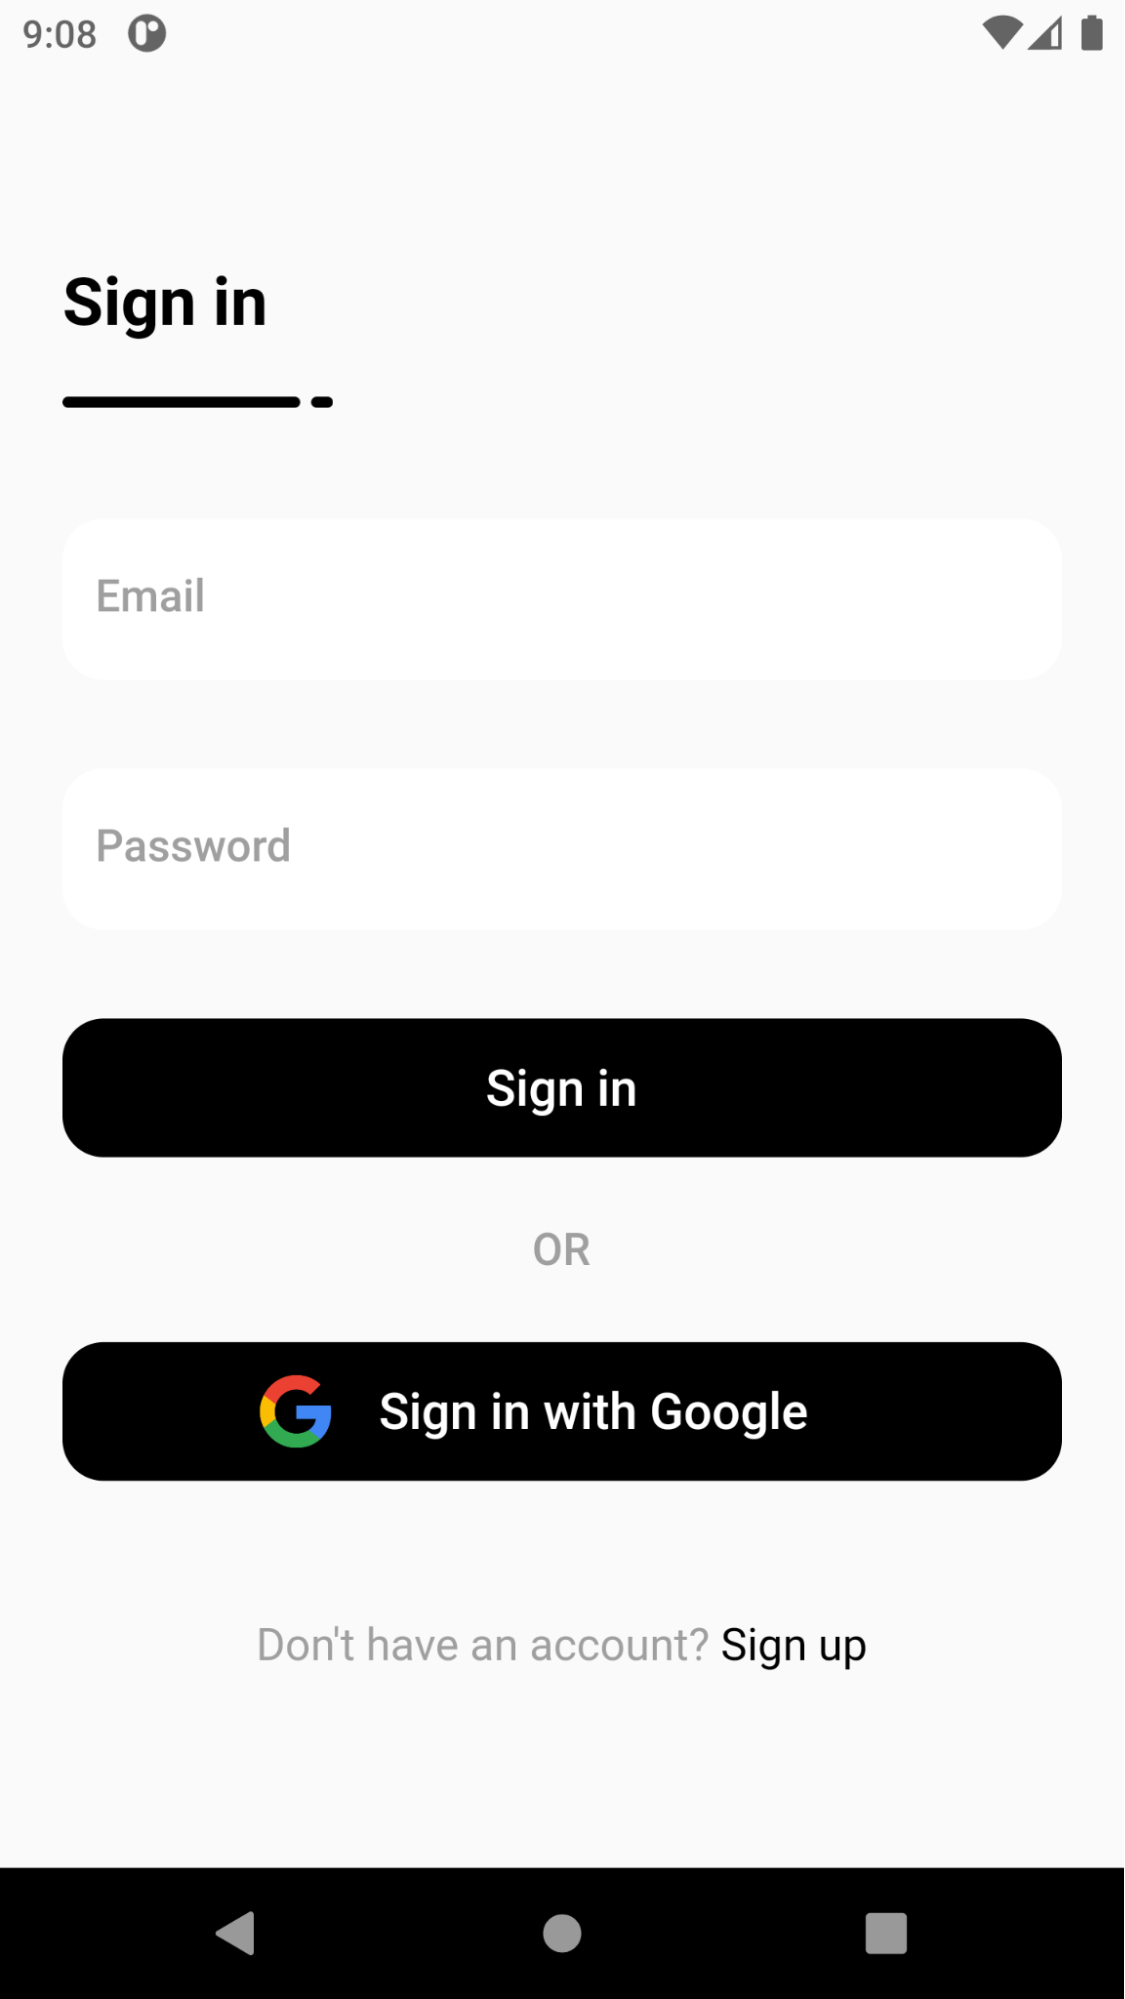
\includegraphics[width=0.5\linewidth]{./images/google.png}
	\caption{Đăng nhập với tài khoản Google}
\end{figure}


Đây là một tính năng vô cùng tiện lợi giúp người dùng có thể sử dụng ngay tài khoản google để đăng nhập vào hệ thống, giảm bớt được phần rườm rà khi phải đăng ký tài khoản mới thì mới có thể sử dụng được hệ thống.
\subsection{Lưu lại cài đặt ngôn ngữ, chủ đề giao diện}
Để thuận tiện cho việc đọc truyện, Honyomi hỗ trợ lưu lại các cài đặt của người dùng về ngôn ngữ hay như chủ đề giao diện nên khi chuyển thiết bị, chỉ cần đăng nhập lại thì các cài đặt sẽ tự động được khôi phục giúp trải nghiệm của người dùng trở nên liền mạch, xuyên suốt hơn.

\begin{figure}[!htb]
	\centering
	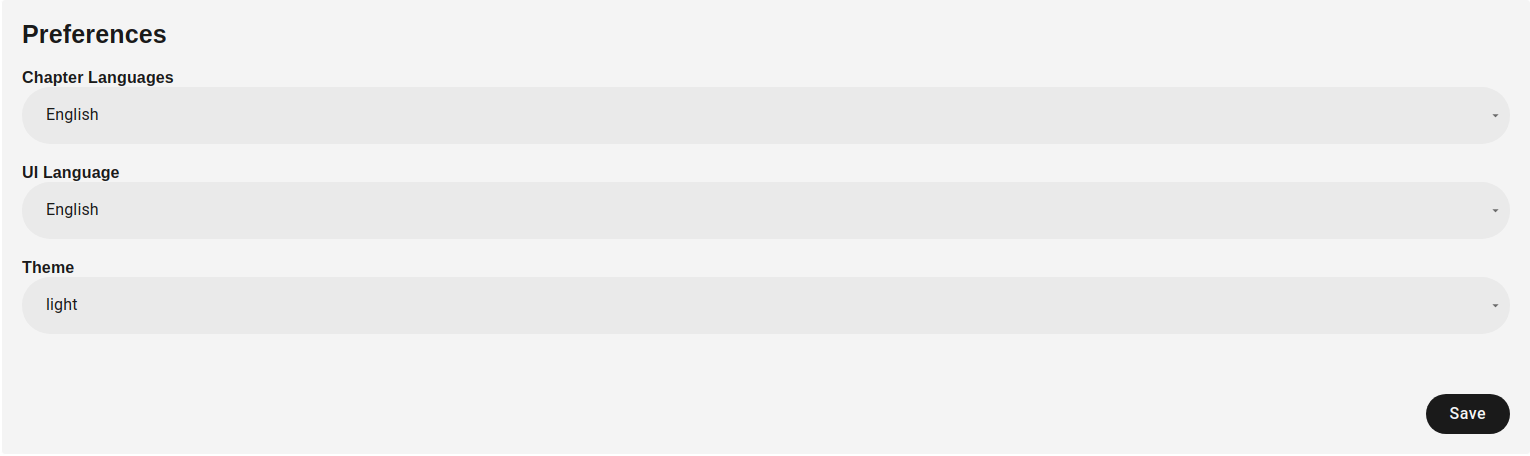
\includegraphics[width=\linewidth]{./images/setting.png}
	\caption{Lưu lại cài đặt}
\end{figure}

\subsection{Gửi mail thông báo khi có chương mới của truyện đang yêu thích}
Là những người đam mê truyện tranh lâu năm, nhóm hiểu được cảm giác muốn được cập nhật nội dung của những bộ truyện mình đang yêu thích. Vì vậy nhóm muốn người dùng của hệ thống có thể nhận được thông tin một cách sớm nhất về nội dung của những bộ truyện họ đang yêu thích ngay khi chúng vừa ra mắt.


\begin{figure}[!htb]
	\centering
	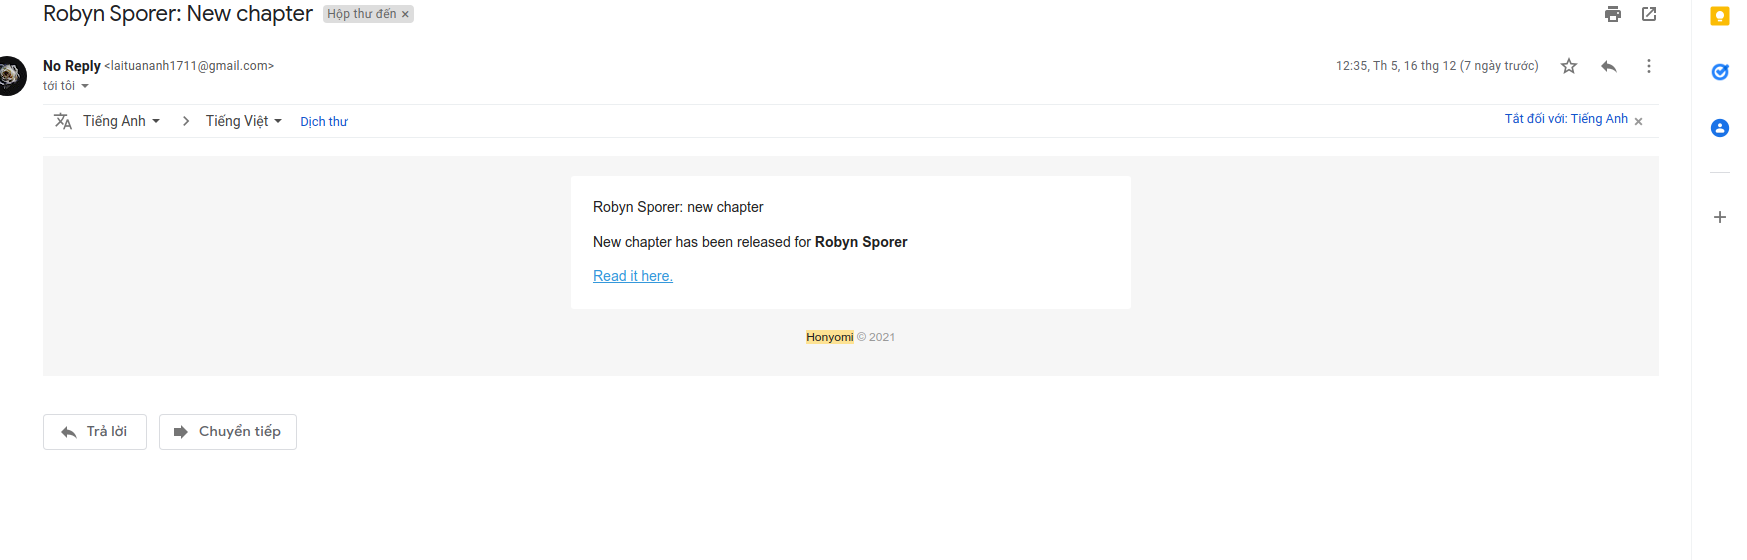
\includegraphics[width=\linewidth]{./images/email.png}
	\caption{Nhận email thông báo}
\end{figure}

\end{document}